\documentclass[12pt,a4paper,dvipdf]{jsarticle}
\usepackage{listings}
\usepackage{amsmath, xparse}
\usepackage{xcolor}
\usepackage[dvipdfmx]{graphicx}
\usepackage{float}
\usepackage{url}
\setlength{\textwidth}{\textwidth}
\setlength{\topmargin}{0pt}
\setlength{\headheight}{0pt}
\setlength{\headsep}{0pt}
\lstset{
    basicstyle = {\ttfamily}, % 基本的なフォントスタイル
    frame = {tbrl}, % 枠線の枠線。t: top, b: bottom, r: right, l: left
    breaklines = true, % 長い行の改行
    numbers = left, % 行番号の表示。left, right, none
    showspaces = false, % スペースの表示
    showstringspaces = false, % 文字列中のスペースの表示
    showtabs = false, % タブの表示
    keywordstyle = \color{blue}, % キーワードのスタイル。intやwhileなど
    commentstyle = {\color[HTML]{1AB91A}}, % コメントのスタイル
    identifierstyle = \color{black}, % 識別子のスタイル 関数名や変数名
    stringstyle = \color{brown}, % 文字列のスタイル
    captionpos = t % キャプションの位置 t: 上、b: 下
}
\title{簡易プロトタイピングによる\\ユーザインタフェース設計\\検討会説明用資料}
\author{202210779 山田 悠真\\202211879 新井 皓陽\\202212115 近 和}
\date{\today}
\begin{document}
\maketitle
\newpage
% \section{sample}
% \begin{figure}[H]
%     \centering
%     \includegraphics[width=10cm]{sample.png}
%     \caption{sample.png}
%     \label{fig:sample}
% \end{figure}


\section{制作するユーザーインターフェースの概要}
\subsection{制作するシステムを選定した経緯}
この課題では「空き教室確認システム」と題して教室の空き状況と設備情報を確認するシステムを作成する。\\
現在存在する学内マップや授業管理システムでは教室に着目したユーザーインターフェースがなく、教室ごとの利用状況を把握することが困難であるため、空き教室を確認するためのユーザーインターフェースを作成することを目標とした。また、学内マップに教室ごとの設備情報が掲載されているが、表形式で纏められているため教室の位置を把握することが困難である。故に、教室の設備情報を教室の位置情報と関連付けたユーザーインターフェースを作成することを目標とした。
\subsection{実験参加者に課す課題内容}
\subsubsection{「現在いる建物の暗幕がある空き教室の場所を見つける」}
詳細
\begin{itemize}
    \item 縁取りされた教室が空き教室である(既知)
    \item 現在いる建物にはマップ上で現在地マーカーを用いて表される
    \item マップ上には教室名とともに利用可能な設備を示すアイコンが配置されている。
\end{itemize}
実験1 : 現在地を3C棟に配置する
実験2 : 現在地を6A棟に配置する

\subsubsection{「条件を満たす部屋の場所を調べる」}
詳細
\begin{itemize}
    \item 課す条件は以下の通り
          \begin{itemize}
              \item 液晶プロジェクターが利用可能
              \item 3C棟に位置する
              \item 1月31日 金曜日の15時15分から18時に空いている
              \item 収容人数が20人以上である
          \end{itemize}
    \item 絞り込み機能を用いることを想定している
\end{itemize}

\subsubsection{「検索窓を用いて特定の教室の利用予定表を確認する」}
詳細
\begin{itemize}
    \item 実験参加者には検索窓を必ず用いる旨を周知する
    \item 検索窓には教室名を入力することのみを想定する
    \item 検索窓に途中まで入力した場合も予測して検索結果を出力する
\end{itemize}
実験1 : 6A202 ビジュアルデザイン室
実験2 : 3A113 計算機室


\section{作成する画面のリストアップ}
\begin{enumerate}
    \item 全学エリアの地図
    \item 第123エリアの地図
    \item 第3エリアの地図
    \item 大学会館・体育・芸術エリアの地図
    \item 3C棟1階の地図
    \item 3C棟2階の地図
    \item 3C棟3階の地図
    \item 3C棟4階の地図
    \item 6A棟1階の地図
    \item 6A棟2階の地図
    \item 6A棟3階の地図
    \item 6A棟4階の地図
    \item 3C113の設備情報と利用予定表
    \item 6A202の設備情報と利用予定表
    \item 検索窓
    \item 検索画面
    \item 絞り込みタブ
    \item エリア選択タブ
    \item 絞り込み結果
\end{enumerate}

\section{作成する画面のデザイン}
\begin{enumerate}
    \item 全学エリアの地図
    \item エリアの地図
    \item 棟の地図
    \item 教室の情報と利用予定表
    \item 検索
    \item エリア選択
    \item 絞り込み
    \item 絞り込み中の地図
\end{enumerate}
\begin{figure}[H]
    \centering
    \begin{minipage}[b]{0.24\columnwidth}
        \centering
        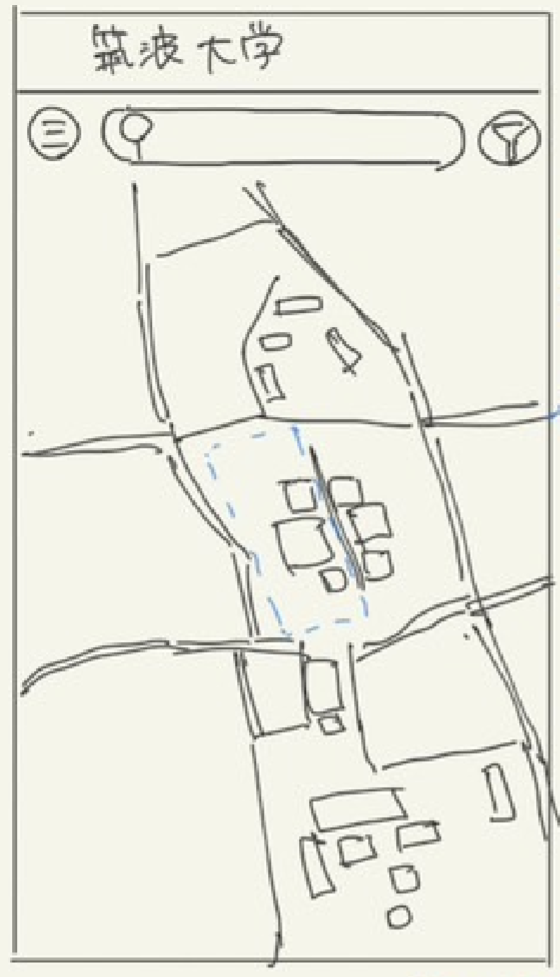
\includegraphics[width=0.9\columnwidth]{./img/全学地図.png}
        \caption{全学地図}
        \label{fig:全学地図}
    \end{minipage}
    \begin{minipage}[b]{0.24\columnwidth}
        \centering
        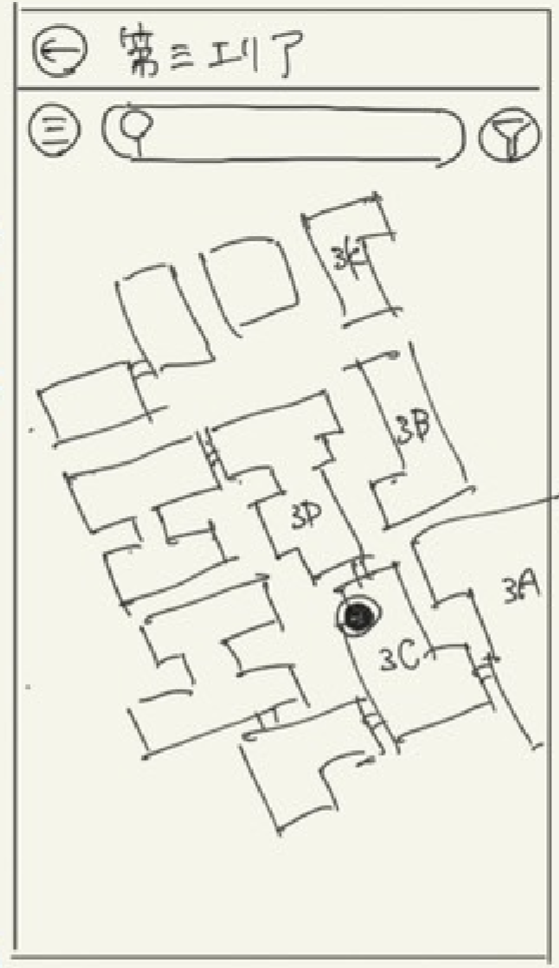
\includegraphics[width=0.9\columnwidth]{./img/エリア地図.png}
        \caption{エリア地図}
        \label{fig:エリア地図}
    \end{minipage}
    \begin{minipage}[b]{0.24\columnwidth}
        \centering
        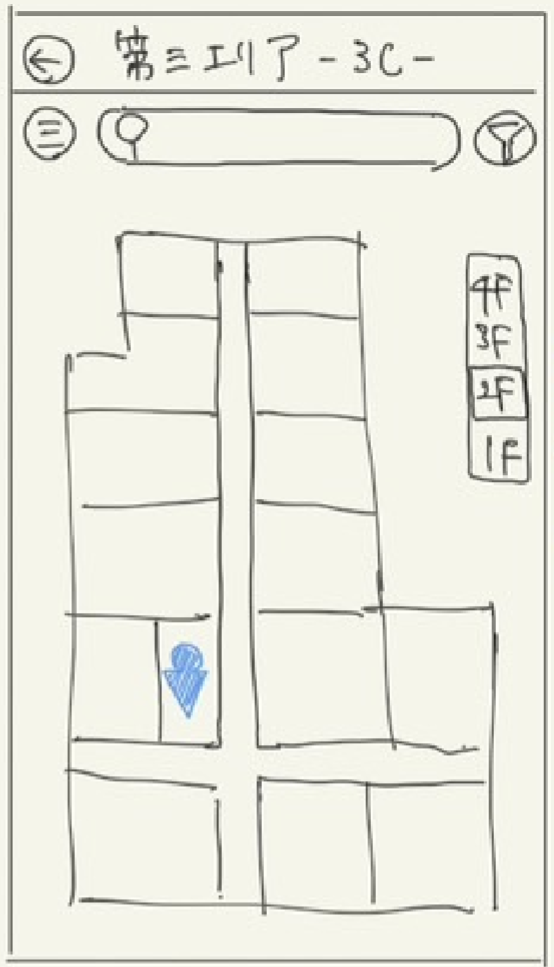
\includegraphics[width=0.9\columnwidth]{./img/棟地図.png}
        \caption{棟地図}
        \label{fig:棟地図}
    \end{minipage}
    \begin{minipage}[b]{0.24\columnwidth}
        \centering
        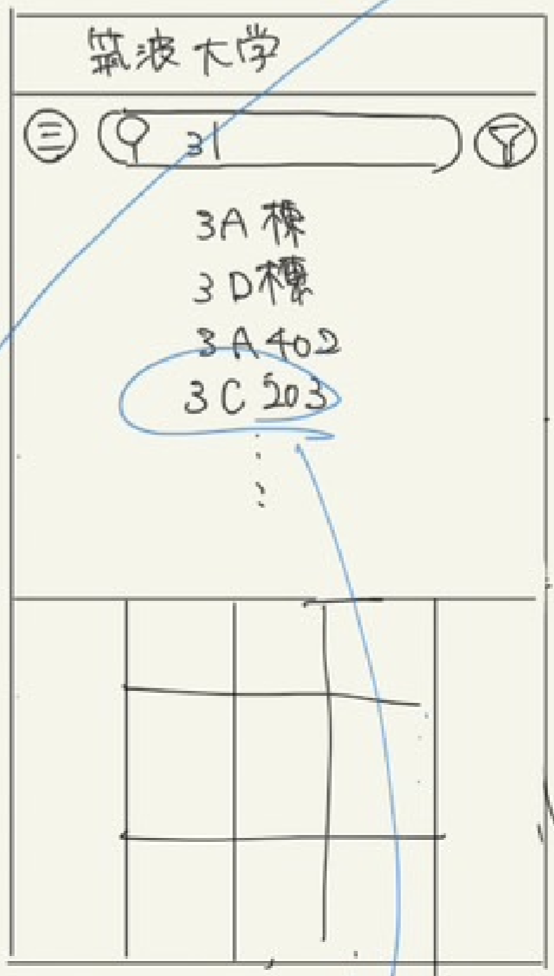
\includegraphics[width=0.9\columnwidth]{./img/検索.png}
        \caption{検索}
    \end{minipage}
\end{figure}
\begin{figure}[H]
    \centering
    \begin{minipage}[b]{0.24\columnwidth}
        \centering
        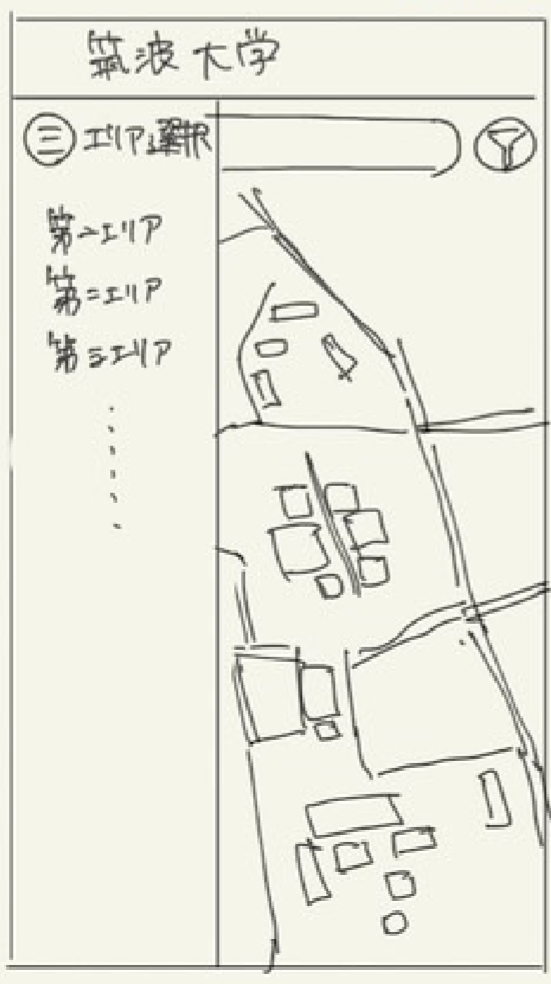
\includegraphics[width=0.9\columnwidth]{./img/エリア選択.png}
        \caption{エリア選択}
    \end{minipage}
    \begin{minipage}[b]{0.24\columnwidth}
        \centering
        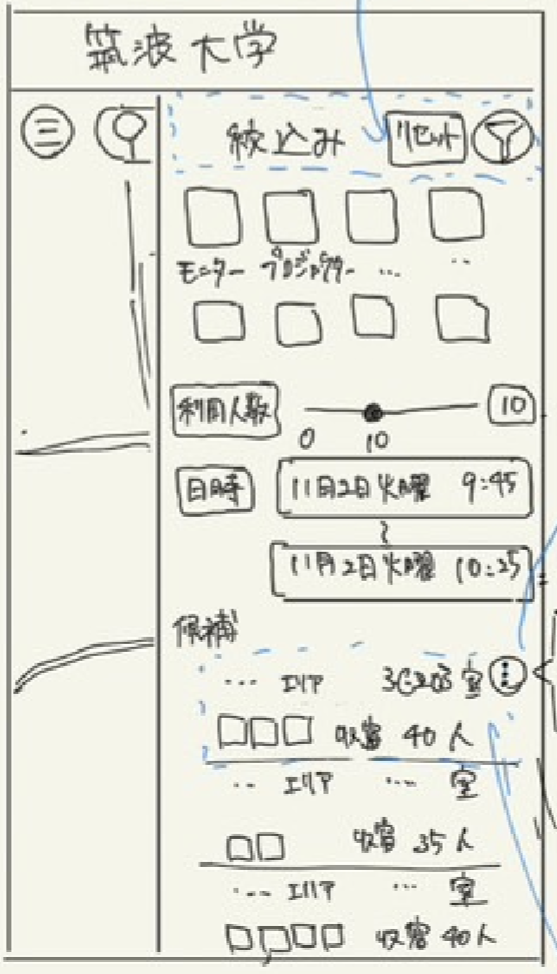
\includegraphics[width=0.9\columnwidth]{./img/絞り込み.png}
        \caption{絞り込み}
    \end{minipage}
    \begin{minipage}[b]{0.24\columnwidth}
        \centering
        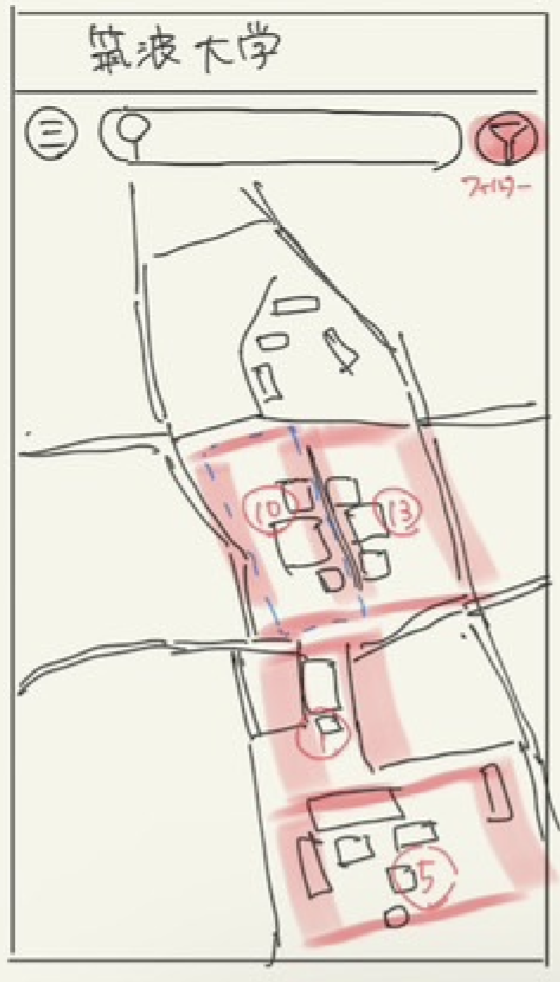
\includegraphics[width=0.9\columnwidth]{./img/絞り込み中.png}
        \caption{絞り込み中}
    \end{minipage}
    \begin{minipage}[b]{0.24\columnwidth}
        \centering
        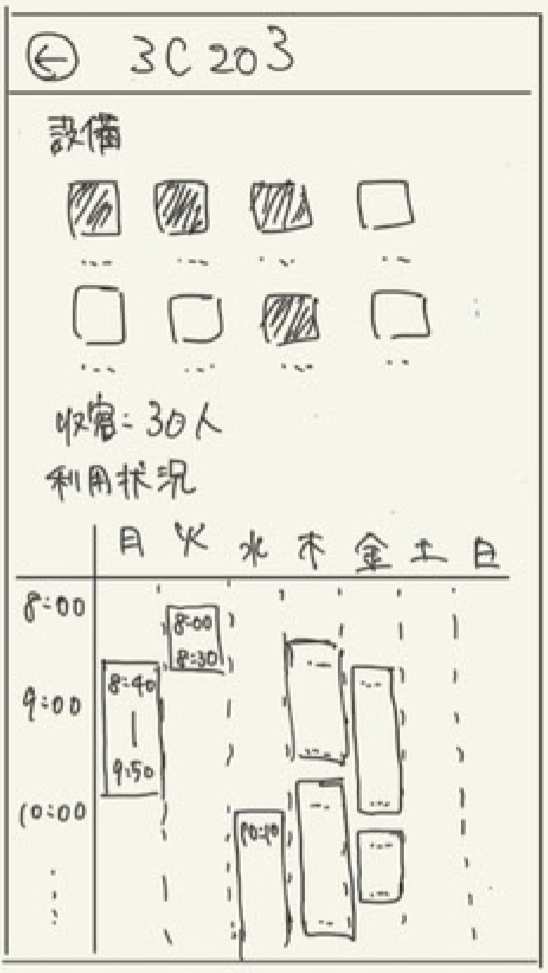
\includegraphics[width=0.9\columnwidth]{./img/部屋情報.png}
        \caption{部屋情報}
    \end{minipage}
\end{figure}



\section{内部的ウォークスルーによる評価}
\subsection{取得するデータ}
\begin{enumerate}
    \item 操作回数
          \begin{itemize}
              \item タップ数
              \item タップした箇所
              \item スクロール数
              \item マップ遷移を行った回数
          \end{itemize}
    \item 実験に要した時間
    \item 実験参加者へのアンケート
          \begin{itemize}
              \item 利用しての感想
              \item アイコンの理解度
              \item 分かりにくい部分
              \item 面倒に感じた部分
          \end{itemize}
\end{enumerate}
\subsection{取得したデータの評価方法}
\subsubsection{KLMを用いて評価する}
\subsubsection{実験参加者へのアンケートの分析}

\section{ユーザビリティテストの準備}
 (実験参加者への指示内容,各役割,観測の方法,試行)
\subsection{実験参加者への指示内容}
\subsubsection{実験参加者に事前に周知する点}
\begin{itemize}
    \item 課題内容
    \item 制作したサービスは空き教室や教室の設備を調べるためのものである
    \item マップの縁取りされている部分は空き教室を示している
    \item 検索バーへの書き込みは入力とみなす
\end{itemize}
\subsection{各役割}
\begin{itemize}
    \item 実験者1(説明係)
          \begin{itemize}
              \item 実験参加者に事前に周知させる事項や実験の課題を説明する
              \item 実験中は他の実験者の補佐を行う
          \end{itemize}
    \item 実験者2(動作係)
          \begin{itemize}
              \item 実験中に実験参加者の操作に応じて画面を切り替える
          \end{itemize}
    \item 実験者3(記録係)
          \begin{itemize}
              \item 操作状況を動画で撮影する
          \end{itemize}
\end{itemize}
\subsection{観測の方法}
\begin{itemize}
    \item スマートフォンで動画を撮影
\end{itemize}
\subsection{試行}
\section{参考文献}
Enhancing KLM (Keystroke-Level Model) to Fit Touch Screen Mobile Devices. Karim El Batran. Mark D. Dunlop. International Conference on Human-Computer Interaction with Mobile Devices and Services, 2014 \\
\url{https://strathprints.strath.ac.uk/49816/1/Karim_MHCI_Final_Camera_Ready.pdf}
\end{document}